\documentclass{bmstu}
\usepackage{bmstu-defabbr}

\usepackage{pdfpages}

\usepackage{listings-rust}
\usepackage{xcolor}
\usepackage{amsmath}

\lstdefinestyle{rust}{
    language=Rust,
    backgroundcolor=\color{white},
    basicstyle=\footnotesize\ttfamily,
    keywordstyle=\color{purple},
    stringstyle=\color{green},
    commentstyle=\color{gray},
    numbers=left,
    stepnumber=1,
    numbersep=5pt,
    frame=single,
    tabsize=4,
    captionpos=t,
    breaklines=true,
    breakatwhitespace=true,
    escapeinside={\#*}{*)},
    morecomment=[l][\color{magenta}]{\#},
    columns=fullflexible
}

\bibliography{biblio}
%\bibliographystyle{utf8gost705u.bst}

\begin{document}

\makecourseworktitle{Информатика, искусственный интеллект и системы управления} % Название факультета
{Программное обеспечение ЭВМ и информационные технологии} % Название кафедры
{Графический редактор композиций тел вращения} % Тема работы
{ИУ7-45Б} % Номер группы
{Романов~С.~К.} % ФИО студента
{Майков~К.~А.} % ФИО научного руководителя
{}
{}


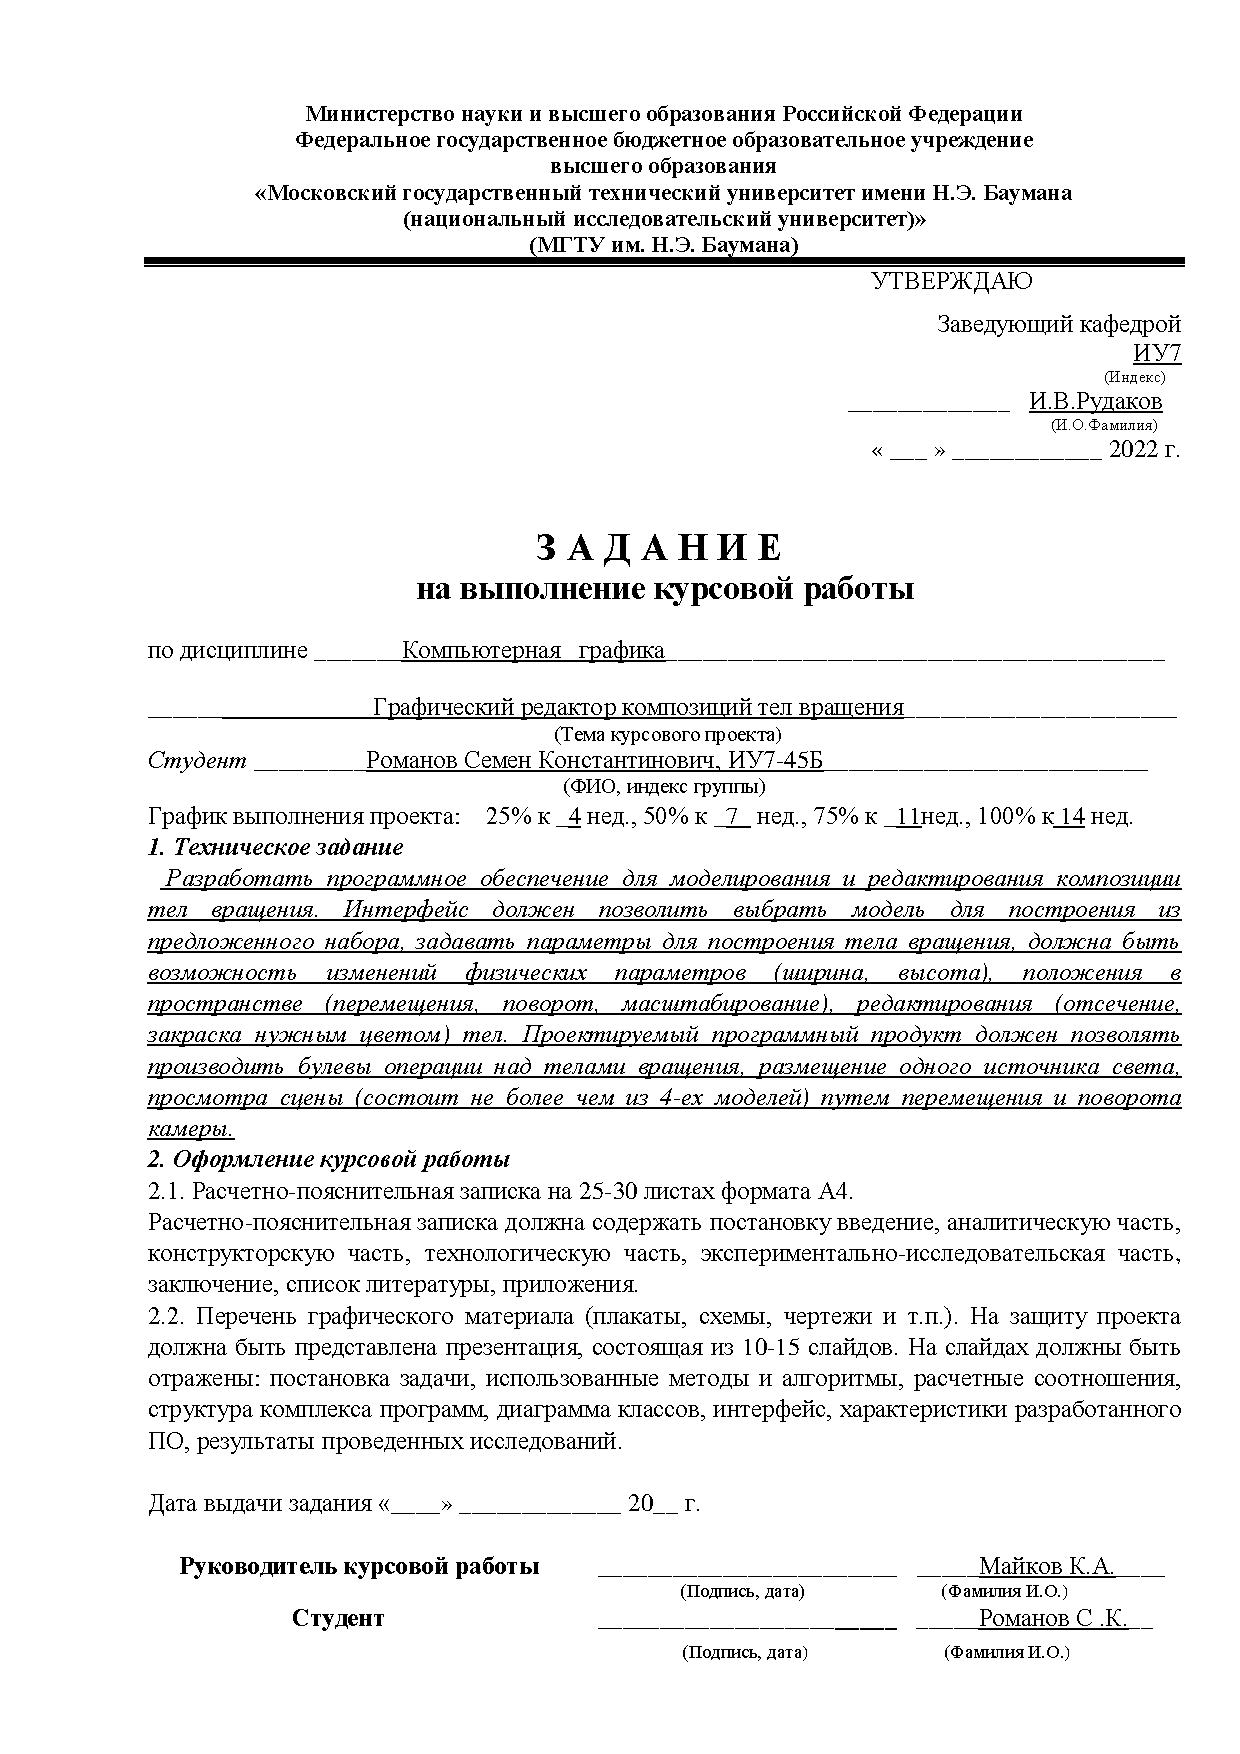
\includepdf[pages={1}]{TZ.pdf}

\maketableofcontents

\begin{definitions}
	\definition{Closed Triangular Irregular Network.}{ Замкнутая ориентированная поверхность,
		разбитая на треугольники со следующими условиями: \newline
		а) каждая точка поверхности принадлежит хотя бы одному треугольнику;\newline
		б) два треугольника могут пересекаться только в одной вершине или по целому ребру. \cite{binary_CTIN}}
	\definition{Constructive Solid Geometry}{ Метод, используемый в твердотельном моделировании.
	Конструктивная геометрия твердого тела позволяет разработчику моделей создавать сложную поверхность
	или объект, используя логические операторы для объединения более простых объектов,
		потенциально создавая визуально сложные объекты путем объединения нескольких примитивных объектов.\cite{binary_Z}}
\end{definitions}
\specsection{ОБОЗНАЧЕНИЯ И СОКРАЩЕНИЯ}
% \addcontentsline{toc}{specsection}{ОБОЗНАЧЕНИЯ И СОКРАЩЕНИЯ}

В настоящей расчетно-пояснительной записке применяют следующие сокращения и обозначения.\\

\begin{description}	
	\item{GUI} --- <<Графический интерфейс пользователя>>.
	\item{ПО} --- Программное обеспечение
\end{description}


\specsection{ВВЕДЕНИЕ}
% \addcontentsline{toc}{specsection}{Введение}
Целью данного курсового проекта является разработка ПО, визуализирующие различные композиции тел вращения.
Это включает в себя такие вещи, как
\begin{enumerate}%[ 1{)}] 
    \item Воссоздание сложных композиций тел.
    \item Создание тел вращения путем вращения выше обозначенных композиций вокруг установленной оси.
    \item Представление полноценной освещенной сцены с композициями объектов.
    \item Обзор рабочей сцены из различных ее участков посредством нескольких камер.
    \item Интерактивность с различными объектами сцены, такими как:
        \begin{itemize}
        \item[$-$] Камеры;
        \item[$-$] Модели;
        \item[$-$] Композиты.
    \end{itemize}
\end{enumerate}
Для достижения поставленных целей необходимо решить следующие задачи:
\begin{itemize}
    \item[$-$] описать структуру трехмерной сцены;
    \item[$-$] реализовать оптимальные алгоритмы представления, преобразования и визуализации твердотельной модели;
    \item[$-$] реализовать аппаратную обработку всех элементов сцены;
    \item[$-$] спроектировать процесс моделирования сцены;
    \item[$-$] описать использующиеся структуры данных;
    \item[$-$] определить средства программной реализации;
    \item[$-$] провести экспериментальные замеры временных характеристик разработанного ПО.
\end{itemize}
В ходе курсовой работы будут затронуты такие темы, как:
\begin{itemize}
    \item[$-$] понятия о телах и поверхностях вращения;
    \item[$-$] удаление невидимых линий и поверхностей;
    \item[$-$] методы закрашивания объемных тел;
    \item[$-$] преимущества и особенности языка Rust.
\end{itemize}

\section{Аналитический раздел}

В данной части проводится анализ объектов сцены и существующих
алгоритмов построения изображений и выбор более подходящих алгоритмов
для дальнейшего использования.
\subsection{Описание объектов сцены}

Сцена состоит из следующих объектов:
\begin{itemize}
    \item[$-$] \textbf{Камера} -- объект, с которого осуществляется наблюдение за сценой. Характеризуется своим пространственным положением, направлением просмотра, углом обзора, ближним и дальним границами обзора.
    \item[$-$] \textbf{Источник света} -- объект, который освещает сцену. Направленный источник света представляет собой вектор направления света и принимает ортогональную проекцию визуализируемой сцены из своего положения с некоторым ограниченным положением. 
В зависимости от расположения источника и направления распространения лучей света, определяется тень от объекта, расположенных на сцене.
    \item[$-$] \textbf{Модель} -- сущность, которая может быть отображена на сцене. Примитивные тела вращения, расположенные в пространстве сцены. Каждая модель представляет собой набор граней, описываемых точками в пространстве, которые соединены ребрами.
    \item[$-$] \textbf{Композит} -- объект, который может содержать в себе другие объекты.
\end{itemize}

\subsection{Анализ методов создания моделей}
Тело вращения — это поверхность в евклидовом пространстве,
образованная вращением кривой (образующей) вокруг оси вращения.\cite{revolution}

На данном этапе стоит рассмотреть существующие схемы представления тел.

\subsubsection{Представление тел вращения}

Тела вращения характеризуются осью, радиусами оснований и конструктивными точками образующей поверхности тел.
Чтобы лучше разобраться в принципах конструктивного построения формы цилиндра и конуса,
следует обратить внимание на рис. \ref{img:tor} и на рис. \ref{img:frame_revol}, где они изображены в виде прозрачных проволочных моделей.
На рисунках ясно выражены конструктивная основа и объемно-пространственная характеристика формы предметов.
Задача состоит в том, чтобы реализовать грамотное и правильное изображение тел на сцене.

\img{60mm}
{tor} % Имя файла без расширения (файл должен быть расположен в директории inc/img/)
{Проволочная модель тора} % Подпись рисунка

\img{100mm}
{frame_revol} % Имя файла без расширения (файл должен быть расположен в директории inc/img/)
{Различные проволочные модели} % Подпись рисунка

Тело вращения образуется вращательной разверткой кривой профиля C вокруг оси. Если поверхность задается с помощью:\newline

\begin{equation}
P(u, v) = (X(v)cos(u), X(v)sin(u), Z(v))
\end{equation}
где X и Z - функции, тогда вектор нормали может быть задан через:\newline

\begin{equation}
n(u, v) = X(v) (Z' (v)cos(u), Z' (v)sin(u), - X' (v))
\end{equation}

где апостроф обозначает первую производную функции.

%\img{100mm}
%{rotate_profile} % Имя файла без расширения (файл должен быть расположен в директории inc/img/)
%{f} % Обтекание (с обтеканием)
%{h} % Положение рисунка (см. wrapfigure из пакета wrapfig)
%{0.5\textwidth} % Ширина рисунка
%{Профиль вращения} % Подпись рисунка

\subsection{Способы описания трехмерных геометрических моделей на сцене}

В компьютерной графики для описание трехмерных геометрических объектов существует три типа моделей: каркасная, поверхностная и твердотельная~\cite{aaymodelmethod}. Использование моделей позволяет правильно отображать форму и размеры объектов сцены.

\begin{itemize}
	\item \textit{Каркасная модель} --- простейший вид моделей, который содержит минимум информации только о вершинах и ребрах объектов. Это моделирование самого низкого уровня, которое имеет ряд серьезных ограничений, большинство из которых возникает из-за недостатка информации о гранях, которые заключены между ребрами. Невозможно выделить внутреннюю и внешнюю область изображения твердого объемного тела. Однако каркасная модель требует меньше памяти и затрат времени на построение, что достаточно пригодна для решения задач, не требующие информации о поверхности объекта (например, если в объекте есть отверстия). Проблемой этой модели заключается в том, что она не позволяет отличить видимые грани от невидимых. Операции по удалению невидимых линий можно выполнить только вручную с применением команд редактирования каждой отдельной линии, но результат работы нарушает каркасную конструкцию, по причине того что линии невидимы в одном случае и видимы в другом.
	Кроме того, каркасная модель не несет информации о поверхностях, ограничивающих форму, что обуславливает невозможность обнаружения нежелательных взаимодействий между гранями объекта~\cite{roders}.
	\item \textit{Поверхностная модель} часто используется в компьютерной графике, кроме содержание информации о вершинах и ребрах, содержит еще информацию о поверхности. При построении поверхностной модели предполагается, что технические объекты ограничены поверхностями, которые отделяют их от окружающей среды. 
	Недостатком поверхностной модели является отсутствие информации о том, с какой стороны поверхности находится материал.
	\item \textit{Твердотельная модель} отличается от поверхностной тем, что в данной модели к информации о поверхностях добавляется информация о том, с какой стороны расположен материал. Это достигается путем указания направления внутренней нормали.
\end{itemize}

Для решения поставленной задачи не подойдет каркасная модель, так как такое представление будет приводить к неправильному восприятию форм объекта. Твердотельная модель также не подойдет, так как по поставленной задачи нет необходимости знать из какого материала будет выполнен тот или иной объект и с какой стороны расположен материал. Поэтому выбор остается лишь поверхностной модели.

\subsection{Способы задания поверхностных моделей}

Поверхностная модель задается следующими способами~\cite{roders, porev}.
\begin{itemize}
	\item \textit{Аналитический (параметрический) способ} характеризуется описанием модели объекта, которое доступно в неявной форме,то есть для получения визуальных характеристик необходимо дополнительно вычислять некоторую функцию, которая зависит от параметра. 
	\item \textit{Полигональная сетка} характеризуется совокупностью вершин, ребер и граней, определяющих форму объекта в трехмерном пространстве.
\end{itemize}

Рассмотрим существующие способы хранения информации о полигональной сетке.

Вершинное представление описывает объект множество вершин, соединенных с другими вершинами (вершины, которые указывают на другие вершины). 
Информация о ребрах и гранях неявно присутствует в представлении из-за чего для восстановления исходного тела необходимо обойти все вершины и составить списки граней. 
Кроме того, операции с ребрами и гранями выполнить нелегко~\cite{aaymodelmethod}.
Тем не менее из-за простоты представления дает возможность множество операций над сеткой. 
Хранение информации о сетке требует не так много памяти по сравнению с другими способами.
На рисунке~\ref{img:vertex-method} представлен пример вершинного представления, рассмотренный на кубе.

\img{100mm}{vertex-method}{Вершинное представление}

Представление называемый списком граней представляет объект не только множеством вершин, но граней. 
В отличие от предыдущего способа, вершины и граны определены явно, благодаря чему нахождение соседних вершин и граней довольно проста и поиск соседних граней и вершин занимает постоянное время~\cite{aaymodelmethod}. 
Также список вершин содержит список граней, связанных с каждой вершиной. 
Однако ребра неявны, поэтому поиск все равно необходим, чтобы найти все грани, окружающие данную грань. 
Другие динамические операции, такие как разделение или слияние граней, также сложны с сетками граней и вершин. 
Пример представления список граней представлен на рисунке~\ref{img:list-faces}.

\img{100mm}{list-faces}{Список граней}

\subsubsection{Понятие поверхности вращения}

Поверхность вращения - это один из часто встречающихся типов поверхностей.
Сферы и цилиндры можно рассматривать как одни из таких аповерхностей.
В общем случае, можно получить тело вращения, вращая тело или набор тел вокруг некоторой произвольной оси.
Чтобы более подробно проанализировать, что это значит, рассмотрим самый простой объект для вращения, а именно точку.
В этом случае получается окружность в плоскости, ортогональной оси, с центром на оси и радиусом,
равным расстоянию точки до оси.\newline

Отсюда следует, что можно представить тело вращения как состоящий из объединения окружностей с центром на оси,
по одной для каждой точки вращаемого объекта.
Это также предполагает, что способ параметризации точки \textbf{P} объекта,
полученного путем вращения кривой вокруг оси, заключается в использовании двух параметров.
Один параметр - это параметр точки на кривой, которая привела к появлению \textbf{P},
а другой - угол, на который она была повернута.
Для общих объектов вращения нам понадобилось бы k + 1 параметров, где k - количество параметров,
необходимых для параметризации вращаемого объекта.

Наше фактическое определение поверхности вращения, которое будет дано в терминах параметризации,
ограничится случаем, когда кривая вращается вокруг оси x.
Это упростит определение. Кроме того, из этого можно получить поверхности вращения вокруг произвольной оси,
используя жесткие движения.

\img{100mm}
{curve} % Имя файла без расширения (файл должен быть расположен в директории inc/img/)
{Поверхность вращения} % Подпись рисунка

\subsubsection{Формализация тела вращения}

Допустим, что
\begin{equation}
g: [a, b] \longrightarrow R^2
\end{equation}

будет плоской параметрической кривой и пусть

\begin{equation}
    g(t) = (g_1(t), g_2(t))
\end{equation}

Определим функцию

\begin{equation}
    p: [a, b] \times [c, d] \longrightarrow R^3
\end{equation}

как

\begin{equation}
    p(t, \theta) = (g_1(t), g_2(t)cos(\theta), g_2(t)sin(\theta))\label{eq:param}
\end{equation}

Подмножество
\begin{equation}
    X = p([a, b] \times [c, d]) \subseteq R^3
\end{equation}
называется поверхностью вращения вокруг оси x для углов c и d относительно g.\newline
Кривые
\begin{equation}
    \gamma(t) = p(t, \theta)
\end{equation}
для фиксированного \(\theta\) являются меридианами поверхности вращения и кривые
\begin{equation}
    \nu(\theta) = p(t, \theta)
\end{equation}
для фиксированного t называются кругами широты.\newline

Используя стандартную параметризацию \(g(t) = (t,f(t))\) для
графика f и замена t на x в уравнении \ref{eq:param}, поверхность, полученная путем вращения графика f вокруг оси x,
параметризуется с помощью формулы

\begin{equation}
    p(x, \theta) = (x, f(x)cos(\theta), f(x)sin(\theta))
\end{equation}

Отсюда легко вычислить производные для этой поверхности

\begin{equation}
    \frac{\delta p}{\delta x} = (1, f'(x)cos(\theta), f'(x)sin(\theta))
\end{equation}
\begin{equation}
    \frac{\delta p}{\delta \theta} = (0, -f(x)sin(\theta), f(x)cos(\theta))
\end{equation}

Из этого можно сразу узнать касательные плоскости в каждой точке,
потому что перекрестное произведение частных производных является нормальным вектором
(при условии, что частные производные не обращаются в нуль).

\subsection{Анализ алгоритмов удаления невидимых линий и поверхностей}

При выборе алгоритма удаления невидимых линий и поверхностей учитывается особенность поставленной
задачи - работа программы будет выполняться в реальном режиме при взаимодействии с пользователем.
Этот факт предъявляет к алгоритму требование по скорости работы.
Для выбора наиболее подходящего алгоритма следует рассмотреть уже имеющиеся алгоритмы удаления невидимых линий и поверхностей.

\subsubsection{Алгоритм обратной трассировки лучей}
Алгоритм работает в пространстве изображения\cite{raytr}.

Суть алгоритма: для определения цвета пиксела экрана через него из точки наблюдения проводится луч,
ищется пересечение первым пересекаемым объектом сцены и определяется освещенность точки пересечения.
Эта освещенность складывается из отраженной и преломленной энергий, полученных от источников света,
а также отраженной и преломленной энергий, идущих от других объектов сцены.
После определения освещенности найденной точки учитывается ослабление света при прохождении через прозрачный материал
и в результате получается цвет точки экрана.

Преимущества:
\begin{itemize}
    \item изображение, которое строится с учётом явлений дисперсии лучей, преломления, а также внутреннего отражения;
    \item возможность использования в параллельных вычислительных системах.
\end{itemize}

Недостатки:
\begin{itemize}
    \item трудоёмкие вычисления\cite{tracer_proof};
\end{itemize}

\subsubsection{Алгоритм, использующий Z-буфер}
Алгоритм работает в пространстве изображения\cite{zbuf}.

Сущность алгоритма: имеется 2 буфера - буфер кадра, который используется для запоминания цвета каждого
пиксела изображения, а также $z$-буфер - отдельный буфер глубины,
используемый для запоминания координаты $z$ (глубины)
каждого видимого пиксела изображения.
В процессе работы глубина или значение $z$ каждого нового пиксела,
который нужно занести в буфер кадра, сравнивается с глубиной того пиксела,
который уже занесен в $z$-буфер.
Если это сравнение показывает, что новый пиксел расположен выше пиксела,
находящегося в буфере кадра ($z > 0$),
то новый пиксел заносится в цвет рассматриваемого пиксела заносится в буфер кадра, а координата $z$ - в $z$-буфер.
По сути, алгоритм является поиском по $x$ и $y$ наибольшего значения функции $z(x, y)$.

Преимущества:
\begin{itemize}
    \item возможность обработки произвольных поверхностей, аппроксимируемых полигонами;
    \item отсутствие требования сортировки объектов по глубине.
\end{itemize}

Недостатки:
\begin{itemize}
    \item отсутствие возможности работы с прозрачными и просвечивающими объектами (в классической версии).
\end{itemize}

\subsubsection{Алгоритм Робертса}
Алгоритм работает в объектном пространстве\cite{robert}.

Суть алгоритма: алгоритм прежде всего удаляет из каждого тела те ребра или грани, которые экранируются самим телом. Затем каждое из видимых ребер каждого тела сравнивается с каждым из оставшихся тел для определения того, какая его часть или части, если таковые есть, экранируются этими телами.

Преимущества:
\begin{itemize}
    \item реализации алгоритма, использующие предварительную приоритетную сортировку вдоль оси z и простые габаритные или минимаксные тесты, демонстрируют почти линейную зависимость от числа объектов\cite{robert}.
\end{itemize}

Недостатки:
\begin{itemize}
    \item вычислительная трудоёмкость алгоритма теоретически растет, как квадрат числа объектов\cite{robert};
    \item отсутствие возможности работы с прозрачными и просвечивающими объектами.
\end{itemize}

\subsubsection*{Вывод}

В таблице \ref{tab:cmp_del} представлено сравнение алгоритмов\cite{rogers} удаления невидимых линий и поверхностей (по каждому параметру составлен рейтинг: 1 - лучший алгоритм, 3 - худший). Так как главным требованием к алгоритму является скорость работы, алгоритмы были оценены по следующим критериям:
\begin{itemize}
    \item скорость работы (С);
    \item масштабируемость с ростом количества моделей (ММ);
    \item масштабируемость с увеличением размера экрана (МЭ);
    \item работа с фигурами вращения (ФВ).
\end{itemize}

\begin{table}[!h]
    \begin{center}
        \begin{tabular}{| @{\hspace{7mm}}r@{\hspace{7mm}} | @{\hspace{7mm}}r@{\hspace{7mm}} | @{\hspace{7mm}}l@{\hspace{7mm}} | @{\hspace{7mm}}l@{\hspace{7mm}} | @{\hspace{7mm}}l@{\hspace{7mm}} |}
            \hline
            Алгоритм & С & ММ & МЭ & ФВ \\
            \hline
            Z-буфера & 1 & 2 & 1 & 1 \\
            Трассировка лучей & 3 & 1 & 3 & 2\\
            Робертса & 2 & 3 & 1 & 3\\
            \hline
        \end{tabular}
    \end{center}
    \caption{\label{tab:cmp_del} Сравнение алгоритмов удаления невидимых линий и поверхностей.}
\end{table}

С учётом результатов в таблице \ref{tab:cmp_del} был выбран алгоритм \textbf{Z-буфера} удаления невидимых линий и поверхностей.

% \subsection{Бинарные операции над телами}
%
% \subsubsection{CTIN}
% Для описания гомогенных объектов можно
% использовать граничную модель, определяя
% границу как множество многоугольников. Частным случаем граничной модели является модель трехмерного тела, у которого граница
% представляет собой замкнутое множество нерегулярных треугольников.
% Замкнутую ориентированную поверхность Р разобьем на треугольники со следующими условиями:
% \begin{enumerate}
%     \item каждая точка поверхности Р принадлежит хотя бы одному треугольнику;
%     \item два треугольника могут пересекаться только в одной вершине или по целому ребру.
% \end{enumerate}
%
% Такую модель будем называть
% CTIN-представлением или CTIN-поверхностью
% (CTIN — closed triangular irregular network).\cite{binary_CTIN}\newline
%
% На рис. \ref{img:triang} изображены верхняя и боковая триангулированные поверхности слоя.
%
% В результате любой булевой операции над двумя CTIN-поверхностями можно получить новую CTIN-поверхность
%
% \img{100mm}
% {triang} % Имя файла без расширения (файл должен быть расположен в директории inc/img/)
% {Триангулированная поверхность слоя} % Подпись рисунка
%
% \img{100mm}
% {triang_hard} % Имя файла без расширения (файл должен быть расположен в директории inc/img/)
% {Сложная триангулированная поверхность} % Подпись рисунка
%
% \subsubsection{Улучшенный Z-буффер}
% Другим подходом является путь улучшенной Z-буфферизации.
% Конструктивная геометрия твердого тела (CSG) - это подход к геометрическому
% моделированию. CSG упорядочивает логические операции и примитивные объекты
% в виде дерева. Узлы (или нетерминалы) дерева представляют
% логические операции, а листья (или терминалы) представляют объекты.
% Логическими операциями, используемыми в CSG, являются объединение (\(\cup\)), пересечение
% (\(\cap\)) и разница (-). Аффинные преобразования, такие как масштабирование, перемещение и поворот,
% также могут быть связаны с каждым узлом дерева. На рис. \ref{img:csg_tree} показан абстрактный объект CSG, заданный в терминах коробок,
% сфер и цилиндров. \cite{binary_Z}
%
% \img{100mm}
% {csg_tree} % Имя файла без расширения (файл должен быть расположен в директории inc/img/)
% {CSG-дерево} % Подпись рисунка
%
% В связи с выбранным ранее алгоритмом удаления невидимых линий в виде Z-буффера, был выбран именно этот способ
%
\subsection{Анализ методов закрашивания}

Методы закрашивания используются для затенения полигонов
(или поверхностей, аппроксимированных полигонами)
в условиях некоторой сцены, имеющей источники освещения.

\subsubsection{Простая закраска}

Суть алгоритма: вся грань закрашивается одним уровнем интенсивности,
который зависит высчитывается по закону Ламберта\cite{rogers}.
При данной закраске все плоскости (в том числе и те,
что аппроксимируют фигуры вращения),
будут закрашены однотонно,
что в случае с фигурами вращения будет давать ложные ребра.

Преимущества:
\begin{itemize}
    \item используется для работы с многогранниками, обладающими преимущественно диффузным отражением.
\end{itemize}

Недостатки:

\begin{itemize}
    \item плохо подходит для фигур вращения: видны ребра.
\end{itemize}

\subsubsection{Закраска по Гуро}
Суть алгоритма: билинейная интерполяция в каждой точке интенсивности освещения в вершинах\cite{lmodels}.

Нормаль к вершине можно найти несколькими способами:
\begin{itemize}
    \item интерполировать нормали прилегающих к вершине граней;
    \item использовать геометрические свойства фигуры (так, например, в случае со сферой ненормированный вектор нормали будет в точности соответствовать вектору от центра сферы до рассматриваемой точки).
\end{itemize}

После нахождения нормали ко всем вершинам находится интенсивность в каждой вершине по закону Ламберта.
Затем алгоритм проходится сканирующими строками по рассматриваемому полигону для всех $y: y \in [y_{min}; y_{max}]$. Каждая сканирующая строка пересекает 2 ребра многоугольника, пусть для определённости это будут ребра через одноименные вершины: $MN$ и $KL$. В точках пересечения высчитывается интенсивность путём интерполяции интенсивности в вершинах.
Так, для точки пересечения с ребром $MN$ интенсивность будет рассчитана как (\ref{for:int_mn}):
\begin{equation}
    \label{for:int_mn}
    I_{MN} = \frac{l_1}{l_0} \cdot I_M + \frac{l_2}{l_0} \cdot I_N
\end{equation}
где $l_1$ - расстояние от точки пересечения до вершины $N$, $l_2$ - расстояние от точки пересечения до вершины $M$, $l_0$ - длина ребра $MN$.
Для точки пересечения сканирующей строки с ребром $KL$ интенсивность высчитывается аналогично.

Далее, после нахождения точек пересечения, алгоритм двигается по $Ox$ от левой точки пересечения $X_{left}$ до правой точки пересечения $X_{right}$ и в каждой точке $\mathcal{X}$ интенсивность рассчитывается как (\ref{for:int_x}):
\begin{equation}
    \label{for:int_x}
    I_{\mathcal{X}} = \frac{\mathcal{X} - X_{left}}{X_{right} - X_{left}} \cdot I_{X_{right}} + \frac{X_{right} - \mathcal{X}}{X_{right} - X_{left}} \cdot I_{X_{left}}
\end{equation}

Преимущества:
\begin{itemize}
    \item преимущественно используется с фигурами вращения с диффузным отражением, аппроксимированными полигонами.
\end{itemize}

Недостатки:
\begin{itemize}
    \item при закраске многогранников ребра могут стать незаметными.
\end{itemize}

\subsubsection{Закраска по Фонгу}
Суть алгоритма: данный алгоритм работает похожим на алгоритм Гуро образом, однако ключевым отличием является то, что интерполируются не интенсивности в вершинах, а нормали\cite{lmodels}. Таким образом, закон Ламберта в данном алгоритме применяется в каждой точке, а не только в вершинах, что делает этот алгоритм гораздо более трудоёмким, однако с его помощью можно гораздо лучше изображаются блики.

Преимущества:
\begin{itemize}
    \item преимущественно используется с фигурами вращения с зеркальным отражением, аппроксимированными полигонами.
\end{itemize}

Недостатки:
\begin{itemize}
    \item самый трудоёмкий алгоритм из рассмотренных\cite{rogers}.
\end{itemize}

\subsubsection*{Вывод}

В таблице \ref{tab:cmp_paint} представлено сравнение алгоритмов\cite{rogers} закраски (по каждому параметру составлен рейтинг: 1 - лучший алгоритм, 3 - худший). Так как требованиями к алгоритму являются высокая скорость работы, а также возможность закраски фигур вращения с диффузными свойствами отражения, алгоритмы были оценены по следующим критериям:
\begin{itemize}
    \item скорость работы (С);
    \item работа с фигурами вращения (ФВ);
    \item работа с фигурами со свойствами диффузного отражения (ДО).
\end{itemize}

\begin{table}[!h]
    \begin{center}
        \begin{tabular}{| @{\hspace{7mm}}r@{\hspace{7mm}} | @{\hspace{7mm}}r@{\hspace{7mm}} | @{\hspace{7mm}}l@{\hspace{7mm}} | @{\hspace{7mm}}l@{\hspace{7mm}} |}
            \hline
            Алгоритм & С & ФВ & ДО \\
            \hline
            Простой & 1 & 3 & 1 \\
            Гуро & 2 & 1 & 1 \\
            Фонга & 3 & 1 & 3 \\
            \hline
        \end{tabular}
    \end{center}
    \caption{\label{tab:cmp_paint} Сравнение алгоритмов закраски.}
\end{table}

С учётом результатов в таблице \ref{tab:cmp_paint} был выбран алгоритм закраски \textbf{Гуро}.

%\subsection{Обработка изображения}
%
%Есть 2 основных варианта обработки изображения: рендеринг на центральном и графическом процессорах.
%Они имеет много общего, но существуют различия, которые оказывают огромное влияние на скорость и качество изображения.
%Рендеринг на базе ЦП является традиционным способом и широко используется.
%Напротив, рендеринг с помощью графических процессоров с годами
%становится все более популярным в сообществе благодаря быстроразвивающемуся миру технологий.
%
%\subsubsection{CPU}
%
%CPU — центральный процессор, это основной компонент компьютера, обрабатывающий инструкции.
%Он выполняет вычисления, действия, запускает программы, включая рендеринг. Центральный процессор постоянно
%принимает ввод от пользователя или активных программ, затем обрабатывает данные и выдает вывод,
%который может быть сохранен приложением или
%отображен на экране.
%
%\subsubsection{GPU}
%
%GPU — графический процессор. Разработан для параллельной обработки трудоёмких вычислительных задач.
%Графический процессор используется в широком спектре приложений, ускоряющих рендеринг 3D-графики.
%Кроме того, этот микропроцессор также используется для разгрузки некоторых задач с центрального процессора,
%что заставляет компьютер работать быстрее.
%
%\subsubsection{Сравнение процессоров}
%Рассмотрим различия процессоров приминительно к рендеру:
%1) главное различие между процессорами CPU и GPU заключается в том,
%как каждый из них выполняет разные задачи;
%2) архитектурно CPU состоит всего из нескольких ядер с большим количеством кэш­памяти, которая может обрабатывать несколько программных
%потоков одновременно, Напротив, графический процессор состоит из сотен
%меньших и более эффективных ядер, которые могут одновременно выполнять
%несколько задач и быстрее обрабатывать изображения;
%3) рендеринг с помощью графического процессора более эффективен с
%точки зрения задач обработки, требующих нескольких параллельных процессов, фактически, рендеринг GPU примерно в 10­100 раз быстрее, чем рендеринг CPU;
%4) GPU позволяет в реальном времени просматривать и манипулировать
%3D моделями, источниками света и проекциями в трех измерениях. Некоторое программное обеспечение для рендеринга, предназначенное только для
%графического процессора, может даже позволить полностью работать в окне
%просмотра с включенным Real Time рендерингом, увеличивая результат и минимизируя возможные ошибки, которые могут возникнуть при рендеринге в
%другой программе. CPU же не позволяет рендерить в реальном времени качественные изображения.
%Изначальная цель заключалась в создании приложения для рендера 3D
%модели в режиме реального времени. Такой сценарий позволяет осуществить
%рендеринг на видеокарте, следовательно, для поставленной задачи следует
%выбрать её, а не CPU

\subsection*{Вывод}

В данном разделе были формально описаны тела и поверхности вращения, их структурные характеристики, по которым эти модели строятся,
были рассмотрены алгоритмы удаления невидимых линий и поверхностей,
методы закрашивания поверхностей.
В качестве алгоритма удаления невидимых линий и поверхностей был выбран алгоритм Z-буфера,
в качестве метода закрашивания был выбран алгоритм закраски Гуро.

\section{Конструкторский раздел}
\subsection{Требования к программному обеспечению}
Программа должна предоставлять доступ к функционалу:
\begin{itemize}
    \item Добавление, удаление объектов/композитов;
    \item Вращение, масштабирование, перемещение объектов/композитов;
    \item Редактирование параметров (ширина, высота) объектов;
    \item Изменение положения источника света;
    \item Редактирование объектов (закраска нужным цветом);
    \item Редактирование композитов;
    \item Передвижение по сцене (перемещение и вращение камеры);
\end{itemize}

К программе предъявляются следующие требования:

\begin{itemize}
    \item время отклика программы должно быть менее 1 секунды для корректной работы в интерактивном режиме;
    \item программа должна корректно реагировать на любые действия пользователя.
\end{itemize}

\subsection{Разработка алгоритмов}

\subsubsection{Алгоритм Z-буфера}
\begin{enumerate}
    \item Всем элементам буфера кадра присвоить фоновое значение
    \item Инициализировать Z буфер минимальными значениями глубины
    \item Выполнить растровую развертку каждого многоугольника сцены:
    \begin{itemize}
        \item[$-$] Для каждого пикселя, связанного с многоугольником вычислить его
        глубину z(x, y)
        \item[$-$] Сравнить глубину пискселя со значением, хранимым в Z буфере.

            Если \(z(x, y) > z\_buf(x, y) \), тогда\newline
            \(z\_buf(x,y) = z(x,y), color(x, y) = colorOfPixel.\)
    \end{itemize}
    \item Отобразить результат.
\end{enumerate}

На рис. \ref{img:z-buffer_algo} изображена схема алгоритма Z-буфера

\img{180mm}
{z-buffer_algo} % Имя файла без расширения (файл должен быть расположен в директории inc/img/)
{Алгоритм Z-буфера} % Подпись рисунка
\clearpage
%
%\subsubsection{Простой метод освещения}
%В простом методе освещения интенсивность рассчитывается по закону Ламберта:
%\[I = I0*cos(\alpha)\] где
%I – результирующая интенсивность света в точке
%I0 – интенсивность источника
%\(\alpha\) – угол между нормалью к поверхности и вектором направления света
\subsubsection{Модифицированный алгоритм, использующий z-буфер}
\begin{enumerate}
    \item Для каждого направленного источника света:
    \begin{enumerate}
        \item[$-$] Инициализировать теневой z-буфер минимальным значением глубины;
        \item[$-$] Определить теневой z-буфер для источника.
    \end{enumerate}
    \item Выполнить алгоритм z-буфера для точки наблюдения. При этом, если
    некоторая поверхность оказалась видимой относительно текущей точки
    наблюдения, то проверить, видима ли данная точка со стороны источников света
    \item Для каждого источника света:
    \begin{enumerate}
        \item[$-$] координаты рассматриваемой точки \((x, y, z)\) линейно преобразовать из вида наблюдателя в координаты
        \((x0, y0, z0)\) на виде из рассматриваемого источника света;
        \item[$-$] cравнить значение \(z\_shadowBuf (x0, y0)\) со значением \(z0(x0, y0)\).
        Если \(z0(x0, y0) < zshadowBuf (x0, y0)\), то пиксел высвечивается с учетом его
        затемнения, иначе точка высвечивается без затемнения
    \end{enumerate}
    \item Отобразить результат.
\end{enumerate}

\subsection{Выбор используемых типов и структур данных}
Для разрабатываемого ПО нужно будет реализовать следующие типы и
структуры данных.
\begin{enumerate}
\item \textbf{Источник света} – направленностью света.
\item \textbf{Сцена} – задается объектами сцены.
\item \textbf{Объекты сцены} – задаются вершинами и гранями.
\item \textbf{Математические абстракции}.
    \begin{enumerate}
        \item[$-$] \textbf{Точка} – хранит координаты x, y, z.
        \item[$-$] \textbf{Вектор} – хранит направление по x, y, z.
        \item[$-$] \textbf{Фигура} – хранит вершины, нормаль, цвет.
    \end{enumerate}
\item \textbf{Интерфейс} – используются библиотечные классы для предоставления доступа к интерфейсу.
\item \textbf{Графический обработчик} - абстрактная структура, выполянющая реализацию алгоритмов.
\item \textbf{Фабрики} для сцены, интерфейса, обработчика - для возможной подмены в ходе разработки или дополнения в дальнейшем.
\item \textbf{Композит} - объект, который будет содержать в себе другие объекты
\end{enumerate}

\chapter{Технологический раздел}

\section{Средства реализации}

Основным языком программирования является мультипарадигменный язык Rust\cite{rust}.
\begin{itemize}
    \item[$-$] Одно из главных достоинств данного языка это гарантия безопасной работы с памятью при помощи системы
    статической проверки ссылок, так называемый Borrow Checker\cite{borrow-checker}.
    \item[$-$] Отсутствие сброщика мусора, как следствие, более экономная работа с ресурсами
    \item[$-$] Встроенный компилятор
    \item[$-$] Кросс-платформенность, от UNIX и MacOS до Web
    \item[$-$] Крайне побдробные коды ошибки и документация от разработчиков языка
    \item[$-$] Важно отметить, что язык программирования Rust сопоставим по скорости с такими языками как С и С++,
    предоставляя в то же время более широкий функционал для тестирования кода и контроля памяти.
\end{itemize}

Также были выбраны следующие библиотеки:
\begin{itemize}
    \item[$-$] В качестве графического интерфейса была выбрана библиотека Slint\cite{slint} (или иначе crate в контексте языка Rust)
    \item[$-$] Для рендера изображения была выбрана библиотека tiny-skia\cite{tiny-skia}, предоставляющий быстрый CPU-рендеринг
    \item[$-$] Помимо этого Slint дает инструментарий для запуска приложения в браузере при непосредственном участии WebAssembly при практически нулевых затратах со стороны программиста.
    \item[$-$] Для тестирования ПО использовались инструменты Cargo\cite{cargo} - пакетного менеджера языка Rust, поставляемого вместе с компилятором из официального источника.
\end{itemize}

Среда разработки:
\begin{itemize}
    \item Работа была проведена в среде разработки CLion\cite{clion} от компании JetBrains\cite{JB}
    \item Дополнительный плагин "Rust" для поддержки синтаксиса языка.
\end{itemize}

\section{Структура классов}

На рисунках \ref{img:classes_A} - \ref{img:classes_B} представлена структура реализуемых классов.

\includeimage
{classes_A} % Имя файла без расширения (файл должен быть расположен в директории inc/img/)
{f} % Обтекание (с обтеканием)
{h} % Положение рисунка (см. wrapfigure из пакета wrapfig)
{0.7\textwidth} % Ширина рисунка
{Структура классов-объектов} % Подпись рисунка

\begin{itemize}
    \item Point – класс точки трехмерного пространства. Хранит координаты в пространстве, владеет методами преобразований точки.
    \item Edge – класс грани. Хранит номера задействованных в грани вершин.
    \item Light – класс источника света.
    \item Model - класс модели. Скрывает конкретную реализацию модели(фигуры) и предоставляет единый интерфейс для работы с ней. Владеет методами преобразования модели, а также методами для получения информации о модели.
    \item Composite - класс композита. Хранит в себе набор моделей, владеет методами для работы с ними.
\end{itemize}

\includeimage
{classes_B} % Имя файла без расширения (файл должен быть расположен в директории inc/img/)
{f} % Обтекание (с обтеканием)
{h} % Положение рисунка (см. wrapfigure из пакета wrapfig)
{0.7\textwidth} % Ширина рисунка
{Структура классов} % Подпись рисунка

\begin{itemize}
    \item Drawer – класс, отвечающий за растеризацию сцены. Хранит полотно для отрисовки. Владеет методами алгоритма теневого z-буфера и формирования объекта для отображения рисунка в главном приложении.
    \item App – точка входа в программу.
    \item Ui - класс, отвечающий за отображение графического интерфейса.
    \item TransformManager – абстракция, содержащия методы трансформмации объектов.
    \item TransformManager - абстракция, содержащия методы загрузки объектов.
    \item Canvas - класс, отвечающий за отображение сцены.
\end{itemize}
\section{Реализация алгоритмов}

В листинге \ref{lst:zBuffer} представлена реализация Z-буффера на языке Rust.
%В листинге \ref{lst:frame_model} представлена реализация проволочной фигуры.

\begin{lstlisting}[style=rust, label=lst:zBuffer, caption={Реализация алгоритма Z-буффера}]
#[derive(Copy, Clone)]
pub struct Vector3D<T> {
    pub x: T,
    pub y: T,
    pub z: T,
}
impl<T> Vector3D<T> {
    pub fn new(x: T, y: T, z: T) -> Vector3D<T> {
        Vector3D {
            x: x,
            y: y,
            z: z,
        }
    }
}
impl<T: NumCast> Vector3D<T> {
    pub fn to<V: NumCast>(self) -> Vector3D<V> {
        Vector3D {
            x: NumCast::from(self.x).unwrap(),
            y: NumCast::from(self.y).unwrap(),
            z: NumCast::from(self.z).unwrap(),
        }
    }
}
impl Vector3D<f32> {
    pub fn norm(self) -> f32 {
        return (self.x*self.x+self.y*self.y+self.z*self.z).sqrt();
    }
    pub fn normalized(self, l: f32) -> Vector3D<f32> {
        return self*(l/self.norm());
    }
}
impl<T: fmt::Display> fmt::Display for Vector3D<T> {
    fn fmt(&self, f: &mut fmt::Formatter) -> fmt::Result {
        write!(f, "({},{},{})", self.x, self.y, self.z)
    }
}
impl<T: Add<Output = T>> Add for Vector3D<T> {
    type Output = Vector3D<T>;
    fn add(self, other: Vector3D<T>) -> Vector3D<T> {
        Vector3D { x: self.x + other.x, y: self.y + other.y, z:  self.z + other.z}
    }
}
impl<T: Sub<Output = T>> Sub for Vector3D<T> {
    type Output = Vector3D<T>;
    fn sub(self, other: Vector3D<T>) -> Vector3D<T> {
        Vector3D { x: self.x - other.x, y: self.y - other.y, z:  self.z - other.z}
    }
}
impl<T: Mul<Output = T> + Add<Output = T>> Mul for Vector3D<T> {
    type Output = T;
    fn mul(self, other: Vector3D<T>) -> T {
        return self.x*other.x + self.y*other.y + self.z*other.z;
    }
}
impl<T: Mul<Output = T> + Copy> Mul<T> for Vector3D<T> {
    type Output = Vector3D<T>;
    fn mul(self, other: T) -> Vector3D<T> {
        Vector3D { x: self.x * other, y: self.y * other, z:  self.z * other}
    }
}
impl<T: Mul<Output = T> + Sub<Output = T> + Copy> BitXor for Vector3D<T> {
    type Output = Vector3D<T>;
    fn bitxor(self, v: Vector3D<T>) -> Vector3D<T> {
        Vector3D { x: self.y*v.z-self.z*v.y, y: self.z*v.x-self.x*v.z, z: self.x*v.y-self.y*v.x}
    }
}
\end{lstlisting}

%\begin{lstlisting}[style=rust, label=lst:frame_model, caption={Реализация проволочной модели}]
%...
%// includes
%...
%#[derive(Clone)]
%pub struct FrameFigure
%{
%    points: Vec<Point>,
%    edges: Vec<Edge>,
%}
%
%#[derive(Clone)]
%pub struct FrameModel
%{
%    figure: Rc<RefCell<FrameFigure>>,
%    transform: Matrix4<f32>,
%}
%
%impl FrameFigure
%{
%    pub fn new() -> FrameFigure
%    {
%        FrameFigure
%        {
%            points: Vec::new(),
%            edges: Vec::new(),
%        }
%    }
%
%    pub fn new_with_points(points: Vec<Point>) -> FrameFigure
%    {
%        FrameFigure
%        {
%            points,
%            edges: Vec::new(),
%        }
%    }
%
%    pub fn new_with_edges(edges: Vec<Edge>) -> FrameFigure
%    {
%        FrameFigure
%        {
%            points: Vec::new(),
%            edges,
%        }
%    }
%
%    pub fn new_with_points_and_edges(points: Vec<Point>, edges: Vec<Edge>) -> FrameFigure
%    {
%        FrameFigure
%        {
%            points,
%            edges,
%        }
%    }
%
%    pub fn get_points(&self) -> &Vec<Point>
%    {
%        &self.points
%    }
%
%    pub fn get_edges(&self) -> &Vec<Edge>
%    {
%        &self.edges
%    }
%
%    pub fn get_points_mut(&mut self) -> &mut Vec<Point>
%    {
%        &mut self.points
%    }
%
%    pub fn get_edges_mut(&mut self) -> &mut Vec<Edge>
%    {
%        &mut self.edges
%    }
%
%    pub fn add_point(&mut self, point: Point)
%    {
%        self.points.push(point);
%    }
%
%    pub fn add_edge(&mut self, edge: Edge)
%    {
%        self.edges.push(edge);
%    }
%
%    pub fn remove_point(&mut self, index: usize)
%    {
%        self.points.remove(index);
%    }
%
%    pub fn remove_edge(&mut self, index: usize)
%    {
%        self.edges.remove(index);
%    }
%
%    pub fn get_point(&self, index: usize) -> &Point
%    {
%        &self.points[index]
%    }
%
%    pub fn get_edge(&self, index: usize) -> &Edge
%    {
%        &self.edges[index]
%    }
%
%    pub fn get_point_mut(&mut self, index: usize) -> &mut Point
%    {
%        &mut self.points[index]
%    }
%
%    pub fn get_edge_mut(&mut self, index: usize) -> &mut Edge
%    {
%        &mut self.edges[index]
%    }
%
%    pub fn get_center(&self) -> Point
%    {
%        let mut max = self.points[0];
%        let mut min = self.points[0];
%
%        for point in &self.points
%        {
%            max = Point::new(max.get_x().max(point.get_x()), max.get_y().max(point.get_y()), max.get_z().max(point.get_z()));
%            min = Point::new(min.get_x().min(point.get_x()), min.get_y().min(point.get_y()), min.get_z().min(point.get_z()));
%        }
%
%        (max + min) / Point::new(2.0, 2.0, 2.0)
%    }
%}
%
%impl FrameModel
%{
%    pub(crate) fn new(figure: Rc<RefCell<FrameFigure>>) -> FrameModel
%    {
%        FrameModel
%        {
%            figure,
%            transform: Matrix4::new(1.0, 0.0, 0.0, 0.0,
%                                    0.0, 1.0, 0.0, 0.0,
%                                    0.0, 0.0, 1.0, 0.0,
%                                    0.0, 0.0, 0.0, 1.0),
%        }
%    }
%}
%
%impl Model for FrameModel
%{
%    type Output = FrameFigure;
%    fn get_model(&self) -> Rc<RefCell<Self::Output>>
%    {
%        self.figure.clone()
%    }
%
%    fn get_center(&self) -> Point {
%        self.figure.borrow().get_center()
%    }
%
%    fn get_transform(&self) -> Matrix4<f32>
%    {
%        self.transform
%    }
%    fn transform(&mut self, transform: Matrix4<f32>) {
%        self.transform = self.transform * transform;
%    }
%}
%
%impl Visibility for FrameModel
%{
%    fn is_visible(&self) -> bool
%    {
%        true
%    }
%}
%\end{lstlisting}
\section*{Вывод}

В данном разделе были рассмотрены средства, с помощью которых было реализовано ПО, а также представлены структуры классов и листинги кода с реализацией алгоритмов компьютерной графики.

%\chapter{Исследовательский раздел}
%\specsection{ЗАКЛЮЧЕНИЕ}
% \addcontentsline{toc}{specsection}{ЗАКЛЮЧЕНИЕ}
Целью данного курсового проекта была достигнута, то есть был разработан программный продукт, позволяющий создавать и редактировать композиции из трехмерных графических тел вращения. Также ПО предоставляет возможности настройки геометрических характеристик объектов, положения камеры и положения источника освещения. 

Для достижение цели были выполнены следующие задачи:
\begin{itemize}
	\item проведен анализ существующих алгоритмов компьютерной графики, использующие для создание реалистичной модели и трехмерной сцены;
	\item выбраны наиболее подходящие алгоритмы (алгоритмы удаления невидимых линий, методы закраски, модели освещения) для решения поставленной задачи;
	\item спроектированы архитектура и графический интерфейс программы;
	\item выбраны средства реализации программного обеспечения;
	\item разработано ПО и реализация выбранных алгоритмов и структур данных;
	\item проведены замеры временных характеристик разработанного программного обеспечения.  
\end{itemize}

В процессе исследовательской работы было выяснено, что полученная модель имеет линейную зависимость времени отрисовки от количества граней и количества объектов. Данное свойство говорит о том, что программа будет хорошо работать со средним количеством объектов, однако для большего их количества понадобятся дополнительные оптимизации вычислений.
В частности, быстродействие низкоуровневых частей программы, отвечающих за растеризацию полигонов, может быть улучшено за счет замены их программной реализации на поддерживаемую аппаратно из интерфейсов графических движков, например, OpenGL или DirectX.


\makebibliography

%\begin{appendices}
	\chapter{}
\end{appendices}

\end{document}
